\documentclass[noauthor,nooutcomes,hints,handout]{ximera}

\graphicspath{  
{./}
{./whoAreYou/}
{./drawingWithTheTurtle/}
{./bisectionMethod/}
{./circles/}
{./anglesAndRightTriangles/}
{./lawOfSines/}
{./lawOfCosines/}
{./plotter/}
{./staircases/}
{./pitch/}
{./qualityControl/}
{./symmetry/}
{./nGonBlock/}
}


%% page layout
\usepackage[cm,headings]{fullpage}
\raggedright
\setlength\headheight{13.6pt}


%% fonts
\usepackage{euler}

\usepackage{FiraMono}
\renewcommand\familydefault{\ttdefault} 
\usepackage[defaultmathsizes]{mathastext}
\usepackage[htt]{hyphenat}

\usepackage[T1]{fontenc}
\usepackage[scaled=1]{FiraSans}

%\usepackage{wedn}
\usepackage{pbsi} %% Answer font


\usepackage{cancel} %% strike through in pitch/pitch.tex


%% \usepackage{ulem} %% 
%% \renewcommand{\ULthickness}{2pt}% changes underline thickness

\tikzset{>=stealth}

\usepackage{adjustbox}

\setcounter{titlenumber}{-1}

%% journal style
\makeatletter
\newcommand\journalstyle{%
  \def\activitystyle{activity-chapter}
  \def\maketitle{%
    \addtocounter{titlenumber}{1}%
                {\flushleft\small\sffamily\bfseries\@pretitle\par\vspace{-1.5em}}%
                {\flushleft\LARGE\sffamily\bfseries\thetitlenumber\hspace{1em}\@title \par }%
                {\vskip .6em\noindent\textit\theabstract\setcounter{question}{0}\setcounter{sectiontitlenumber}{0}}%
                    \par\vspace{2em}
                    \phantomsection\addcontentsline{toc}{section}{\thetitlenumber\hspace{1em}\textbf{\@title}}%
                     }}
\makeatother



%% thm like environments
\let\question\relax
\let\endquestion\relax

\newtheoremstyle{QuestionStyle}{\topsep}{\topsep}%%% space between body and thm
		{}                      %%% Thm body font
		{}                              %%% Indent amount (empty = no indent)
		{\bfseries}            %%% Thm head font
		{)}                              %%% Punctuation after thm head
		{ }                           %%% Space after thm head
		{\thmnumber{#2}\thmnote{ \bfseries(#3)}}%%% Thm head spec
\theoremstyle{QuestionStyle}
\newtheorem{question}{}



\let\freeResponse\relax
\let\endfreeResponse\relax

%% \newtheoremstyle{ResponseStyle}{\topsep}{\topsep}%%% space between body and thm
%% 		{\wedn\bfseries}                      %%% Thm body font
%% 		{}                              %%% Indent amount (empty = no indent)
%% 		{\wedn\bfseries}            %%% Thm head font
%% 		{}                              %%% Punctuation after thm head
%% 		{3ex}                           %%% Space after thm head
%% 		{\underline{\underline{\thmname{#1}}}}%%% Thm head spec
%% \theoremstyle{ResponseStyle}

\usepackage[tikz]{mdframed}
\mdfdefinestyle{ResponseStyle}{leftmargin=1cm,linecolor=black,roundcorner=5pt,
, font=\bsifamily,}%font=\wedn\bfseries\upshape,}


\ifhandout
\NewEnviron{freeResponse}{}
\else
%\newtheorem{freeResponse}{Response:}
\newenvironment{freeResponse}{\begin{mdframed}[style=ResponseStyle]}{\end{mdframed}}
\fi



%% attempting to automate outcomes.

%% \newwrite\outcomefile
%%   \immediate\openout\outcomefile=\jobname.oc
%% \renewcommand{\outcome}[1]{\edef\theoutcomes{\theoutcomes #1~}%
%% \immediate\write\outcomefile{\unexpanded{\outcome}{#1}}}

%% \newcommand{\outcomelist}{\begin{itemize}\theoutcomes\end{itemize}}

%% \NewEnviron{listOutcomes}{\small\sffamily
%% After answering the following questions, students should be able to:
%% \begin{itemize}
%% \BODY
%% \end{itemize}
%% }
\usepackage[tikz]{mdframed}
\mdfdefinestyle{OutcomeStyle}{leftmargin=2cm,rightmargin=2cm,linecolor=black,roundcorner=5pt,
, font=\small\sffamily,}%font=\wedn\bfseries\upshape,}
\newenvironment{listOutcomes}{\begin{mdframed}[style=OutcomeStyle]After answering the following questions, students should be able to:\begin{itemize}}{\end{itemize}\end{mdframed}}



%% my commands

\newcommand{\snap}{{\bfseries\itshape\textsf{Snap!}}}
\newcommand{\flavor}{\link[\snap]{https://snap.berkeley.edu/}}
\newcommand{\mooculus}{\textsf{\textbf{MOOC}\textnormal{\textsf{ULUS}}}}


\usepackage{tkz-euclide}
\tikzstyle geometryDiagrams=[rounded corners=.5pt,ultra thick,color=black]
\colorlet{penColor}{black} % Color of a curve in a plot



\ifhandout\newcommand{\mynewpage}{\newpage}\else\newcommand{\mynewpage}{}\fi


\title{Symmetries of the square}
\author{Bart Snapp}

\begin{document}
\begin{abstract}
  We explore the symmetries of the regular rectangle, also known as a
  square.
\end{abstract}
\maketitle

\begin{listOutcomes}
\item Witness the symmetries of the square.
\item Describe symmetries of the square.
\item Think of the symmetries of the square as functions.
\item Use the algebra of symmetries to understand a composition of
  symmetries.
\end{listOutcomes}


\begin{listObjectives}
 \item Use mathematical language to describe symmetries.
 \item Take a solution to a problem in a given context, and applying that same solu- tion to another problem
 \item Increase student confidence in their ability to solve difficult math problems by using previous results, trying different methods, asking questions, and working with others.
\item Improve student’s mathematical communication skills.
\end{listObjectives}
\mynewpage


\begin{question}
  The \textbf{symmetries} of the square are those that \textbf{leave
    it unchanged}. So for example, here is a symmetry of the square:
  \[
  \raisebox{-.4\height}{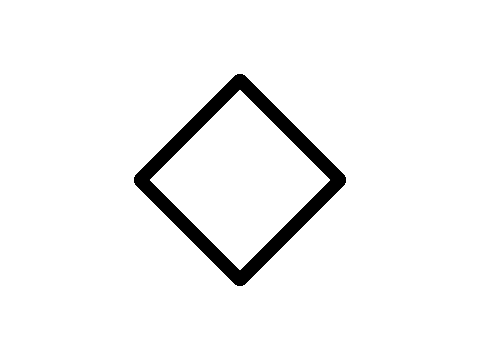
\includegraphics[width=2.5in]{blackSymSquare.png}}\resizebox{.7in}{!}{$\mapsto$} \raisebox{-.4\height}{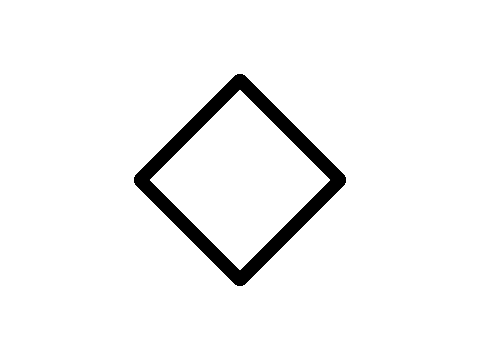
\includegraphics[width=2.5in]{blackSymSquare.png}}
  \]
  You may think nothing happened above, because the triangle is
  unchanged, but you would be wrong.  To WITNESS symmetries, we must
  color-in the sides of the square. For example once I color in the
  sides, we see that the symmetry above is actually:
  \[
  \raisebox{-.4\height}{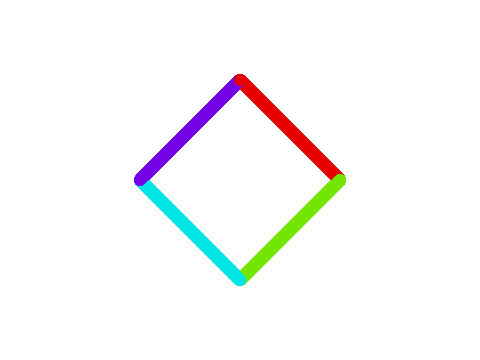
\includegraphics[width=2.5in]{eSq.png}}\resizebox{.7in}{!}{$\mapsto$} \raisebox{-.4\height}{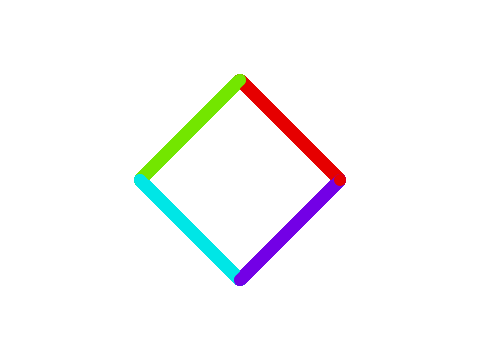
\includegraphics[width=2.5in]{rfSq.png}}
  \]
  While the colors change, the ACTUAL SQUARE is \textbf{unchanged}.
  \begin{enumerate}
  \item What physical action would cause the square to change the colors the way?
  \item What other physical actions are symmetries of an square?
  \item How many symmetries does the square have?
  \end{enumerate}
  \begin{freeResponse}
    \begin{enumerate}
      \item There are EIGHT symmetries of the square.
      \item Here they are: \begin{enumerate}
      \item $\raisebox{-.4\height}{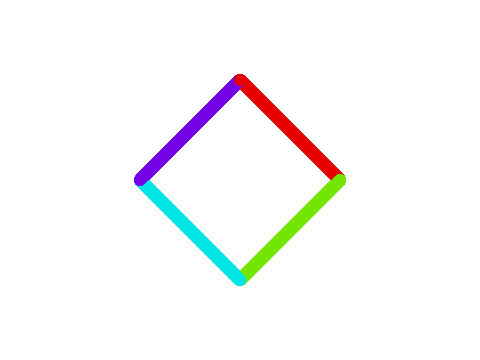
\includegraphics[width=2in]{eSq.png}}\resizebox{.5in}{!}{$\mapsto$} \raisebox{-.4\height}{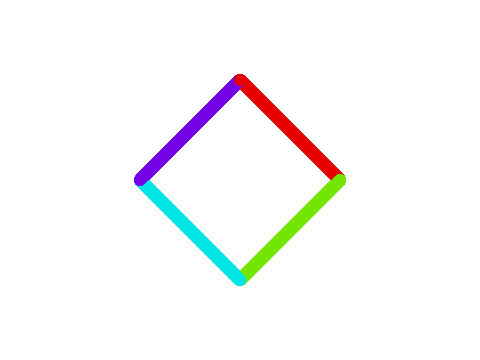
\includegraphics[width=2in]{eSq.png}}$
      \item $\raisebox{-.4\height}{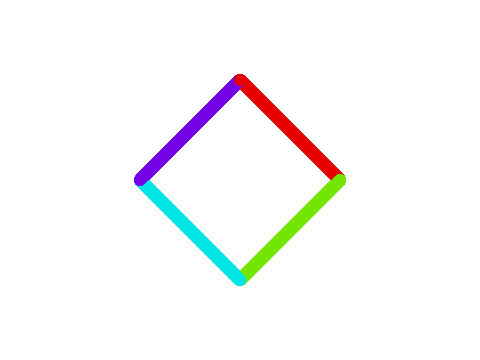
\includegraphics[width=2in]{eSq.png}}\resizebox{.5in}{!}{$\mapsto$} \raisebox{-.4\height}{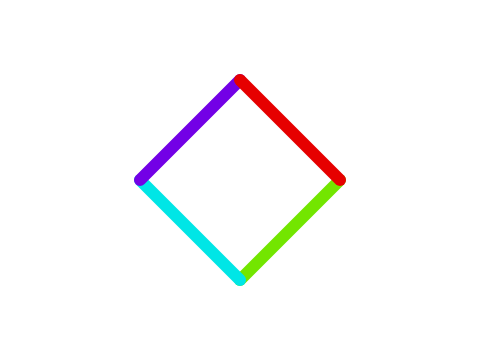
\includegraphics[width=2in]{rSq.png}}$
      \item $\raisebox{-.4\height}{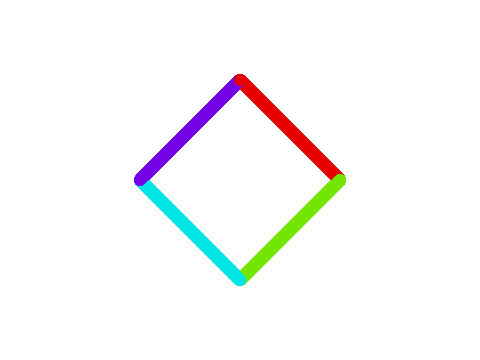
\includegraphics[width=2in]{eSq.png}}\resizebox{.5in}{!}{$\mapsto$} \raisebox{-.4\height}{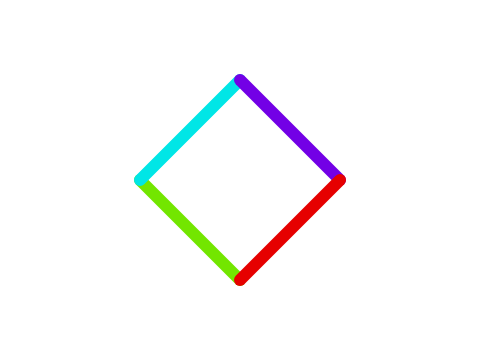
\includegraphics[width=2in]{r2Sq.png}}$
      \item $\raisebox{-.4\height}{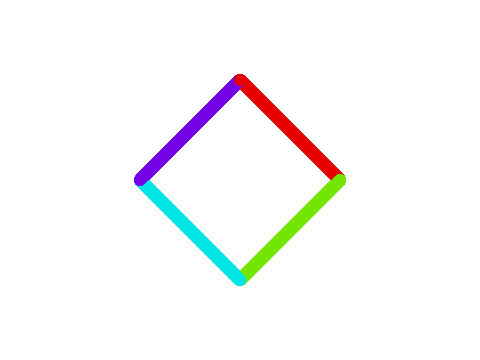
\includegraphics[width=2in]{eSq.png}}\resizebox{.5in}{!}{$\mapsto$} \raisebox{-.4\height}{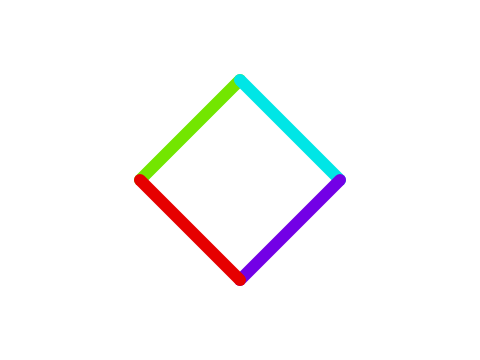
\includegraphics[width=2in]{r3Sq.png}}$
      \item $\raisebox{-.4\height}{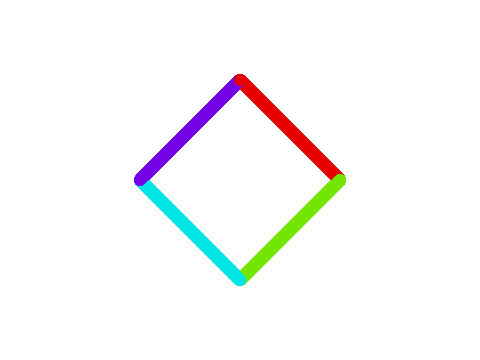
\includegraphics[width=2in]{eSq.png}}\resizebox{.5in}{!}{$\mapsto$} \raisebox{-.4\height}{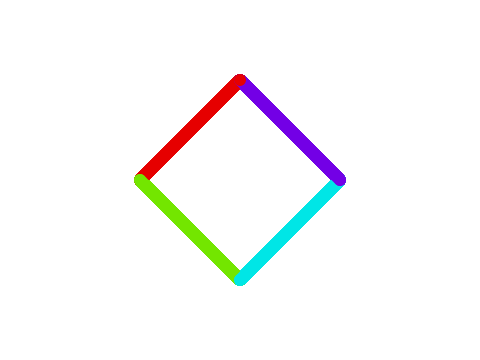
\includegraphics[width=2in]{fSq.png}}$
      \item $\raisebox{-.4\height}{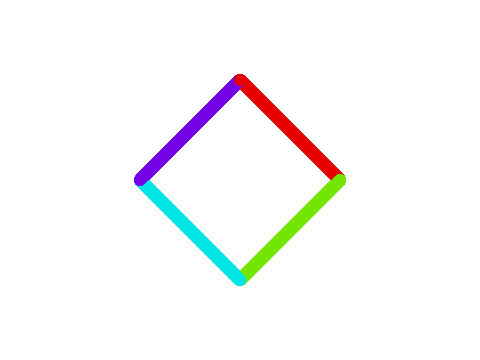
\includegraphics[width=2in]{eSq.png}}\resizebox{.5in}{!}{$\mapsto$} \raisebox{-.4\height}{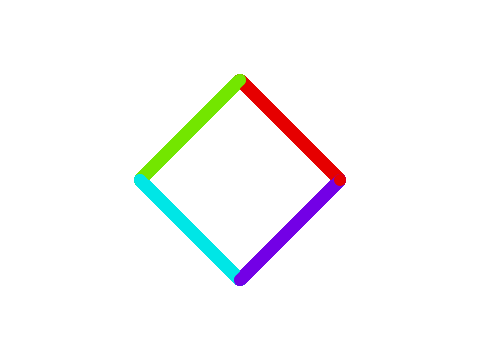
\includegraphics[width=2in]{rfSq.png}}$
      \item $\raisebox{-.4\height}{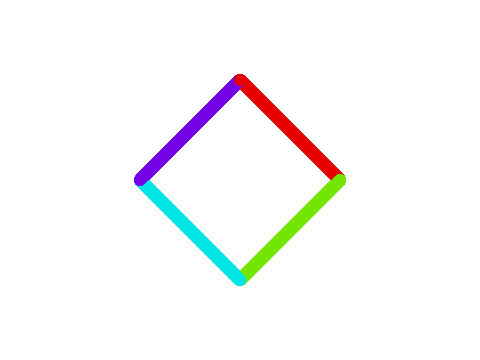
\includegraphics[width=2in]{eSq.png}}\resizebox{.5in}{!}{$\mapsto$} \raisebox{-.4\height}{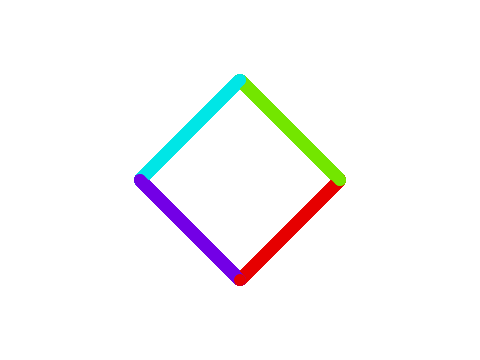
\includegraphics[width=2in]{r2fSq.png}}$
      \item $\raisebox{-.4\height}{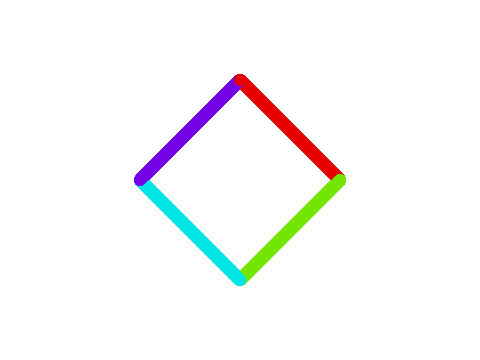
\includegraphics[width=2in]{eSq.png}}\resizebox{.5in}{!}{$\mapsto$} \raisebox{-.4\height}{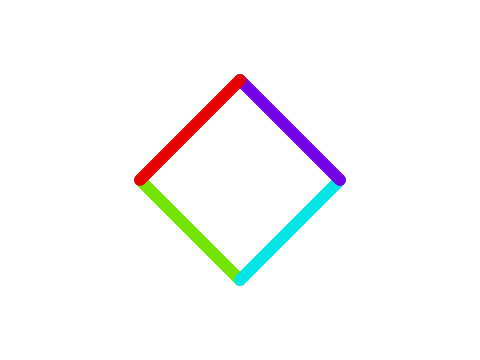
\includegraphics[width=2in]{r3fSq.png}}$
      \end{enumerate}
    \end{enumerate}
  \end{freeResponse}
\end{question}
\mynewpage

\begin{question}
  Let $e$ be the do-nothing symmetry, $r$ be a clockwise $90^\circ$
  rotation about the center of the square, and $f$ be a flip across
  a vertical line down the middle of the square.  When $e$ is
  applied, the triangle looks like this:
  \[
  \raisebox{-.4\height}{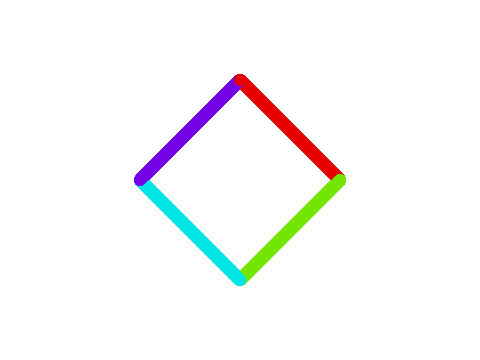
\includegraphics[width=2.5in]{eSq.png}}\resizebox{.7in}{!}{$\overset{\scriptscriptstyle e}{\mapsto}$} \raisebox{-.4\height}{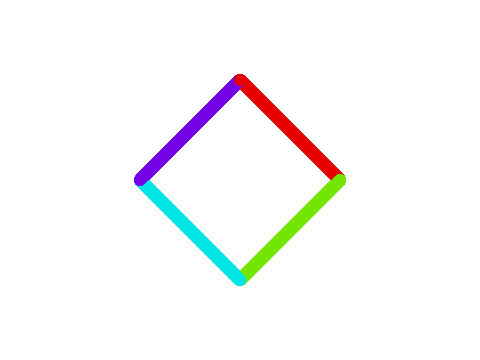
\includegraphics[width=2.5in]{eSq.png}}
  \]
  Display the result of applying the following functions
  (actions/transformations) to your square:
  \begin{enumerate}
  \item $fr$
  \item $r^2 f$
  \item $f r^2$
  \item $r^3 f$
  \end{enumerate}
 In each case, show off your work using colors, numbering, or some other description.
  
  \textbf{WARNING:} Unlike multiplication with numbers, changing the order gives different answers.
  \begin{freeResponse}
    \begin{enumerate}
    \item For $fr$ I have
      \[
      \raisebox{-.4\height}{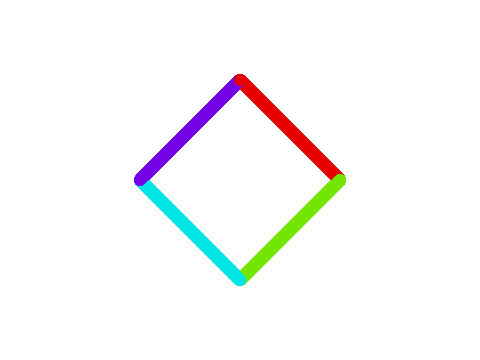
\includegraphics[width=2.5in]{eSq.png}}\resizebox{.7in}{!}{$\overset{\scriptscriptstyle fr}{\mapsto}$} \raisebox{-.4\height}{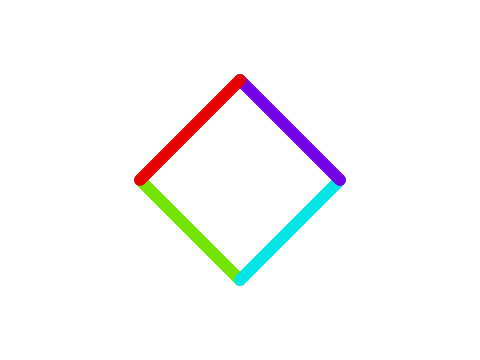
\includegraphics[width=2.5in]{r3fSq.png}}
      \]
    \item For $r^2f$ I have
      \[
      \raisebox{-.4\height}{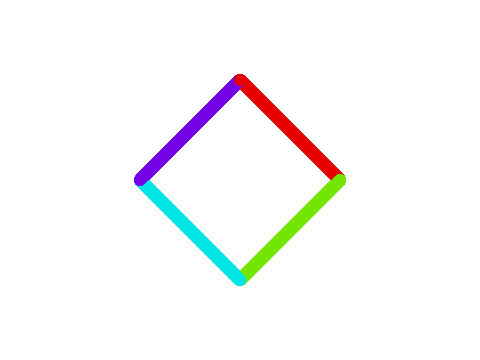
\includegraphics[width=2.5in]{eSq.png}}\resizebox{.7in}{!}{$\overset{\scriptscriptstyle r^2f}{\mapsto}$} \raisebox{-.4\height}{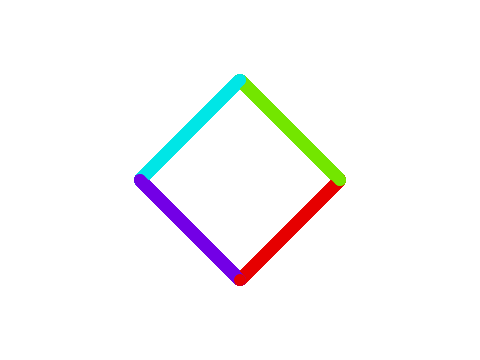
\includegraphics[width=2.5in]{r2fSq.png}}
      \]
    \item For $fr^2$ I have
      \[
      \raisebox{-.4\height}{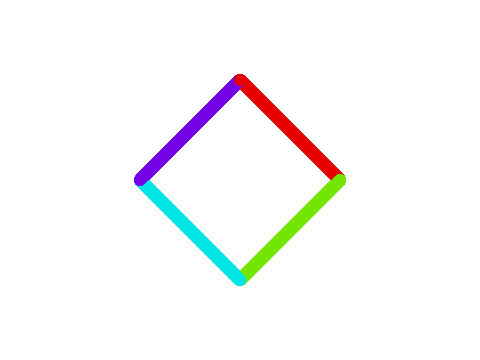
\includegraphics[width=2.5in]{eSq.png}}\resizebox{.7in}{!}{$\overset{\scriptscriptstyle  fr^2}{\mapsto}$} \raisebox{-.4\height}{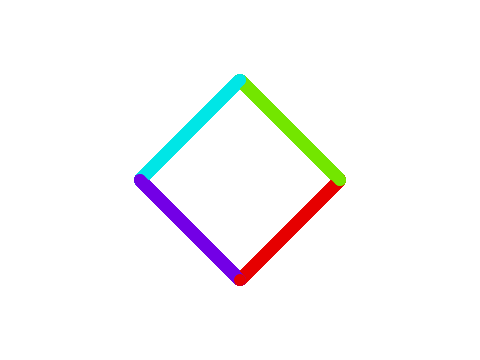
\includegraphics[width=2.5in]{r2fSq.png}}
      \]
    \item For $r^3f$ I have
      \[
      \raisebox{-.4\height}{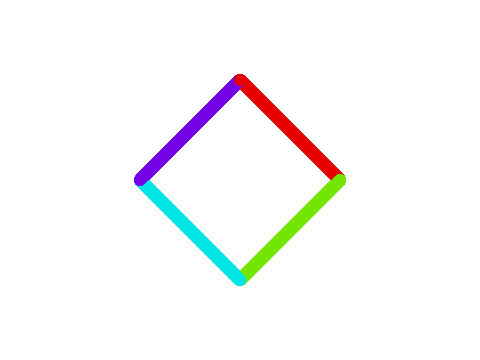
\includegraphics[width=2.5in]{eSq.png}}\resizebox{.7in}{!}{$\overset{\scriptscriptstyle r^3f}{\mapsto}$} \raisebox{-.4\height}{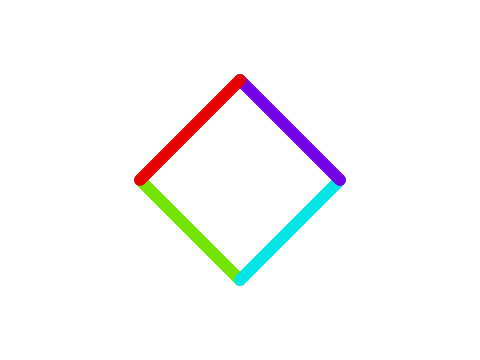
\includegraphics[width=2.5in]{r3fSq.png}}
      \]
    \end{enumerate}
    \end{freeResponse}
\end{question}
\mynewpage


\begin{question}
  Do you remember the MULTIPLICATION TABLES? We can make a similar
  table for the symmetries of the square. Here, I've started it for
  you:
  \[
  \begin{array}{|c||c|c|c|c|c|c|c|c|}
    \hline
         & e    & r     & r^2     & r^3      & f      & rf     & r^2f      &  r^3 f\\ \hline\hline
    e    & e    & r     & r^2     & r^3      & f      & rf     & r^2f      &  r^3 f\\ \hline
    r    & r    & r^2   & r^3     & \color{red}r^4      & rf     & r^2f   & r^3f      & \color{red}r^4f\\ \hline
    r^2  & r^2  & r^3   & \color{red}r^4     & \color{red}r^5      & r^2f   & r^3f   & \color{red}r^4f      & \color{red}r^5f\\ \hline
    r^3  & r^3  & \color{red}r^4   & \color{red}r^5     & \color{red}r^6      & r^3f   & \color{red}r^4f   & \color{red}r^5f      & \color{red}r^6f\\ \hline
    f    & f    & \color{red}fr    & \color{red}fr^2    & \color{red}fr^3     & \color{red}f^2    & \color{red}frf    & \color{red}fr^2f     & \color{red}fr^3f\\ \hline
    rf   & rf   & \color{red}rfr   & \color{red}rfr^2   & \color{red}rfr^3    & \color{red}rf^2   & \color{red}rfrf   & \color{red}rfr^2f    & \color{red}rfr^3f\\ \hline
    r^2f & r^2f & \color{red}r^2fr & \color{red}r^2fr^2 & \color{red}r^2fr^3  & \color{red}r^2f^2 & \color{red}r^2frf & \color{red}r^2fr^2f  & \color{red}r^2fr^3f\\ \hline
    r^3f & r^3f & \color{red}r^3fr & \color{red}r^3fr^2 & \color{red}r^3fr^3  & \color{red}r^3f^2 & \color{red}r^3frf & \color{red}r^3f r^2f & \color{red}r^3fr^3f\\ \hline
  \end{array}
  \]
  Each of the symmetries in red is actually equal to one of the
  symmetries in top row (or left-most column)
  \[
  e,\quad r,\quad r^2,\quad r^3,\quad f,\quad rf,\quad r^2f,\quad r^3f
  \]
  where $e$ is the ``do-nothing'' symmetry.
  \begin{enumerate}
    \item Simplify each of the red symmetries as one of
      $e,r,r^2,f,rf,r^2f$ and update the table with these values.
    \item Use your table to express
      \[
      f^3r^5f^7r^9
      \]
      as one of $e,r,r^2,r^3,f,rf,r^2f, r^3f$.
  \end{enumerate}
  \begin{freeResponse}
    \begin{enumerate}
      \item Here is my updated table:
  \[
  \begin{array}{|c||c|c|c|c|c|c|c|c|}
    \hline
         & e    & r     & r^2     & r^3      & f      & rf     & r^2f      &  r^3 f\\ \hline\hline
    e    & e    & r     & r^2     & r^3      & f      & rf     & r^2f      &  r^3 f\\ \hline
    r    & r    & r^2   & r^3     & e        & rf     & r^2f   & r^3f      & f\\ \hline
    r^2  & r^2  & r^3   & e       & r        & r^2f   & r^3f   &    f      & r  f\\ \hline
    r^3  & r^3  & e     & r       & r^2      & r^3f   &    f   & r  f      & r^2f\\ \hline
    f    & f    & r^3f  & r^2f    & rf       & e      & r^3    & r^2       & r    \\ \hline
    rf   & rf   &  f    & r^3f    & r^2f     & r      & e      & r^3       & r^2   \\ \hline
    r^2f & r^2f & r f   & f       & r^3f     & r^2    & r      & e         & r^3     \\ \hline
    r^3f & r^3f & r^2f  & rf      & f        & r^3    & r^2    & r         & e       \\ \hline
  \end{array}
  \]
\item Using the table I see
  \begin{align*}
    f^3r^5f^7r^9 &= frfr\\
    &= r^3f^2r\\
    &= e.
  \end{align*}
    \end{enumerate}
  \end{freeResponse}
\end{question}
\end{document}
